\section{Research Topics, Challenges, and New Ideas}

% bedk - \par at end ensures proper line spacing
\begin{frame}
  \begin{center}
    {\color{Maroon}\Huge Research Directions and New Modeling Techniques\par}
  \end{center}
\end{frame}

%%%% ----------------------------
%%%%     CHALLENGES
%%%% ----------------------------

\begin{frame}
  \begin{center}
    {\color{Maroon}\Huge Challenges}
  \end{center}
\end{frame}

\begin{frame}{Are we there yet?}
  \begin{center}
    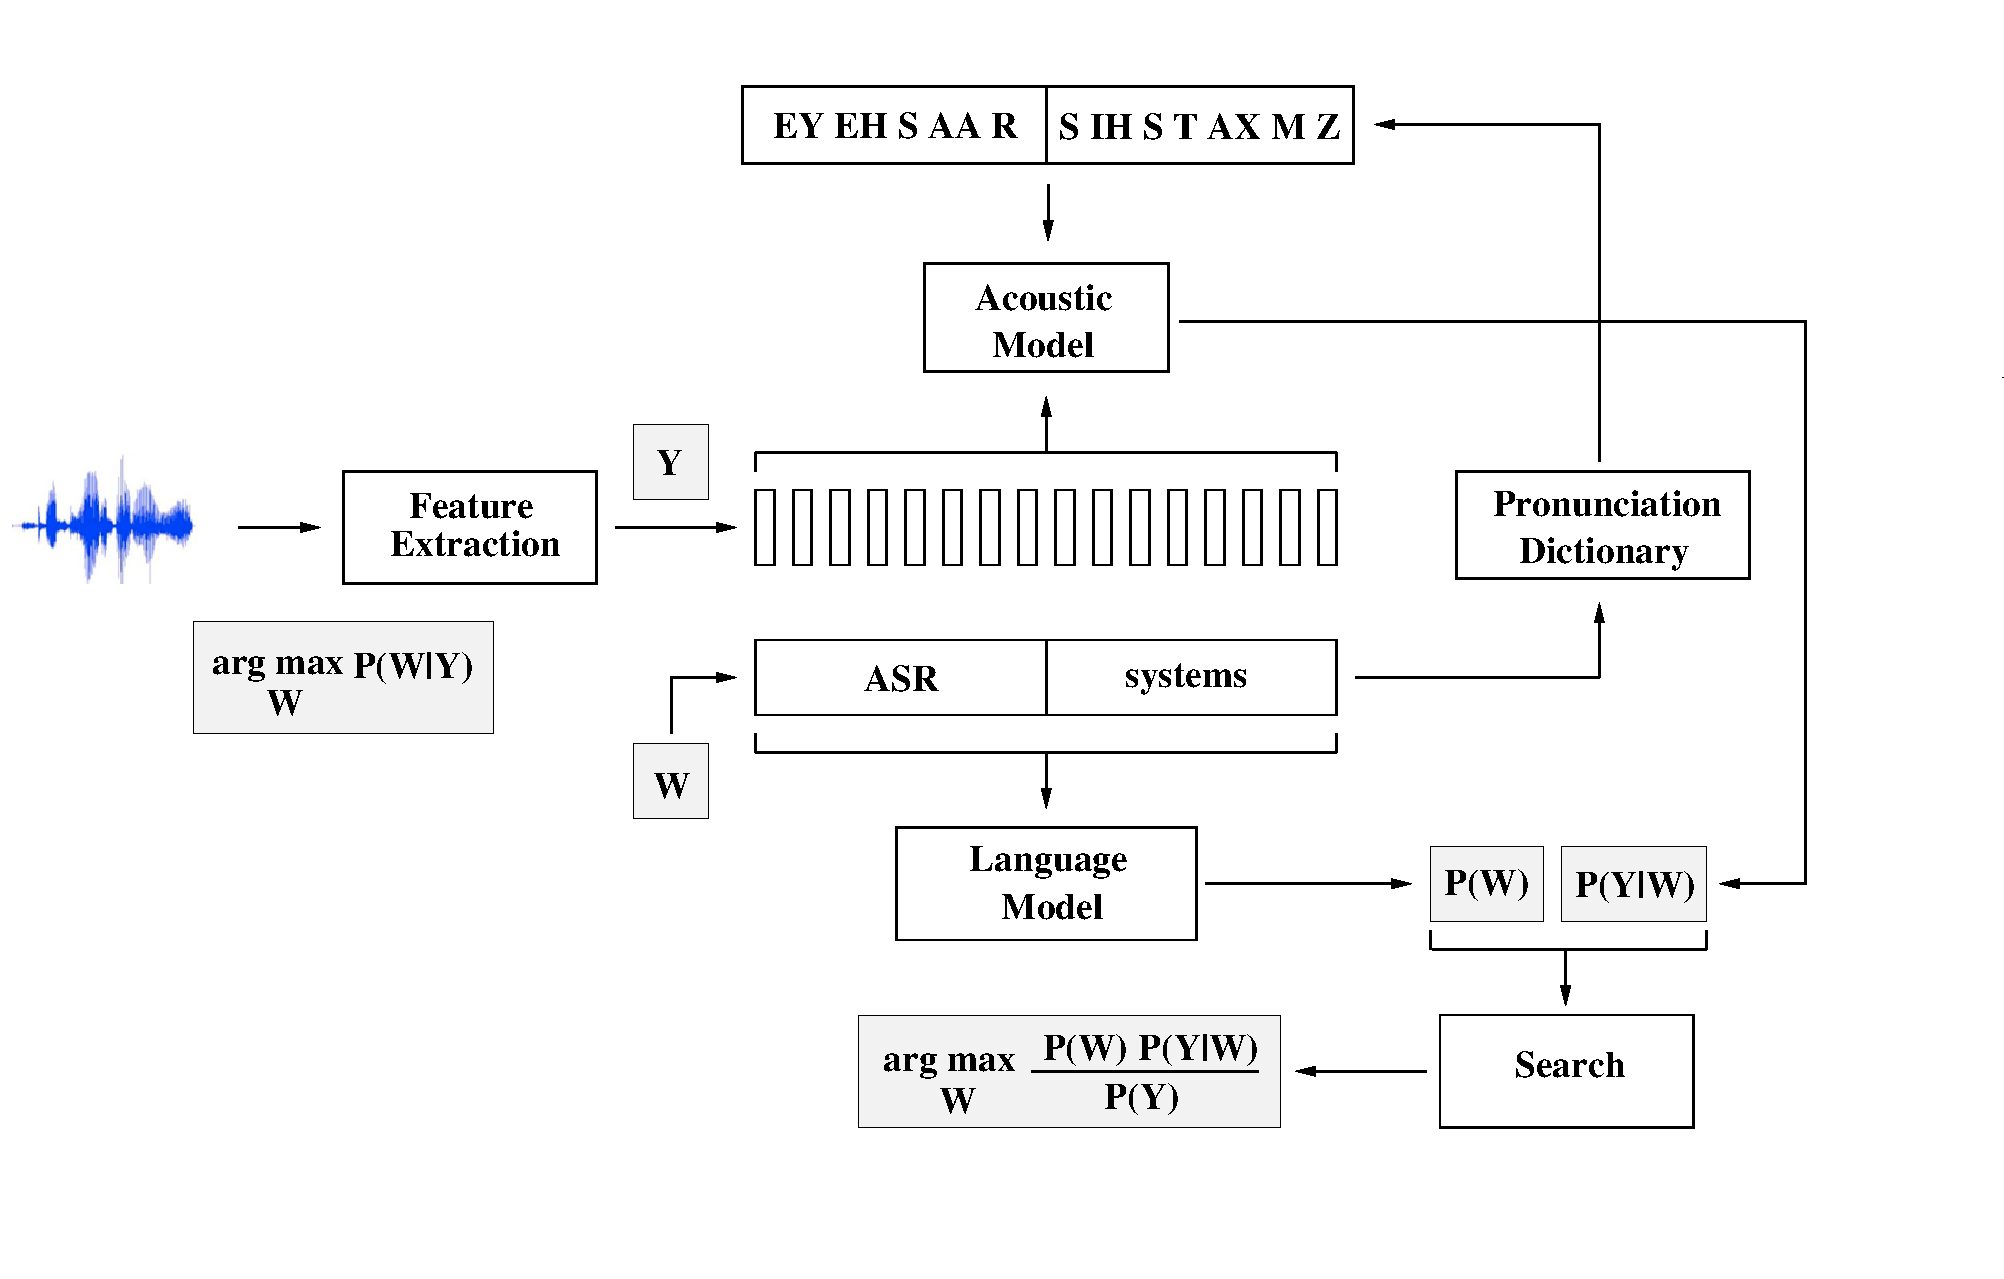
\includegraphics[height=65mm]{figures/ASR9}
  \end{center}
\end{frame}

\begin{frame}{Is that it?}
  \begin{center}
    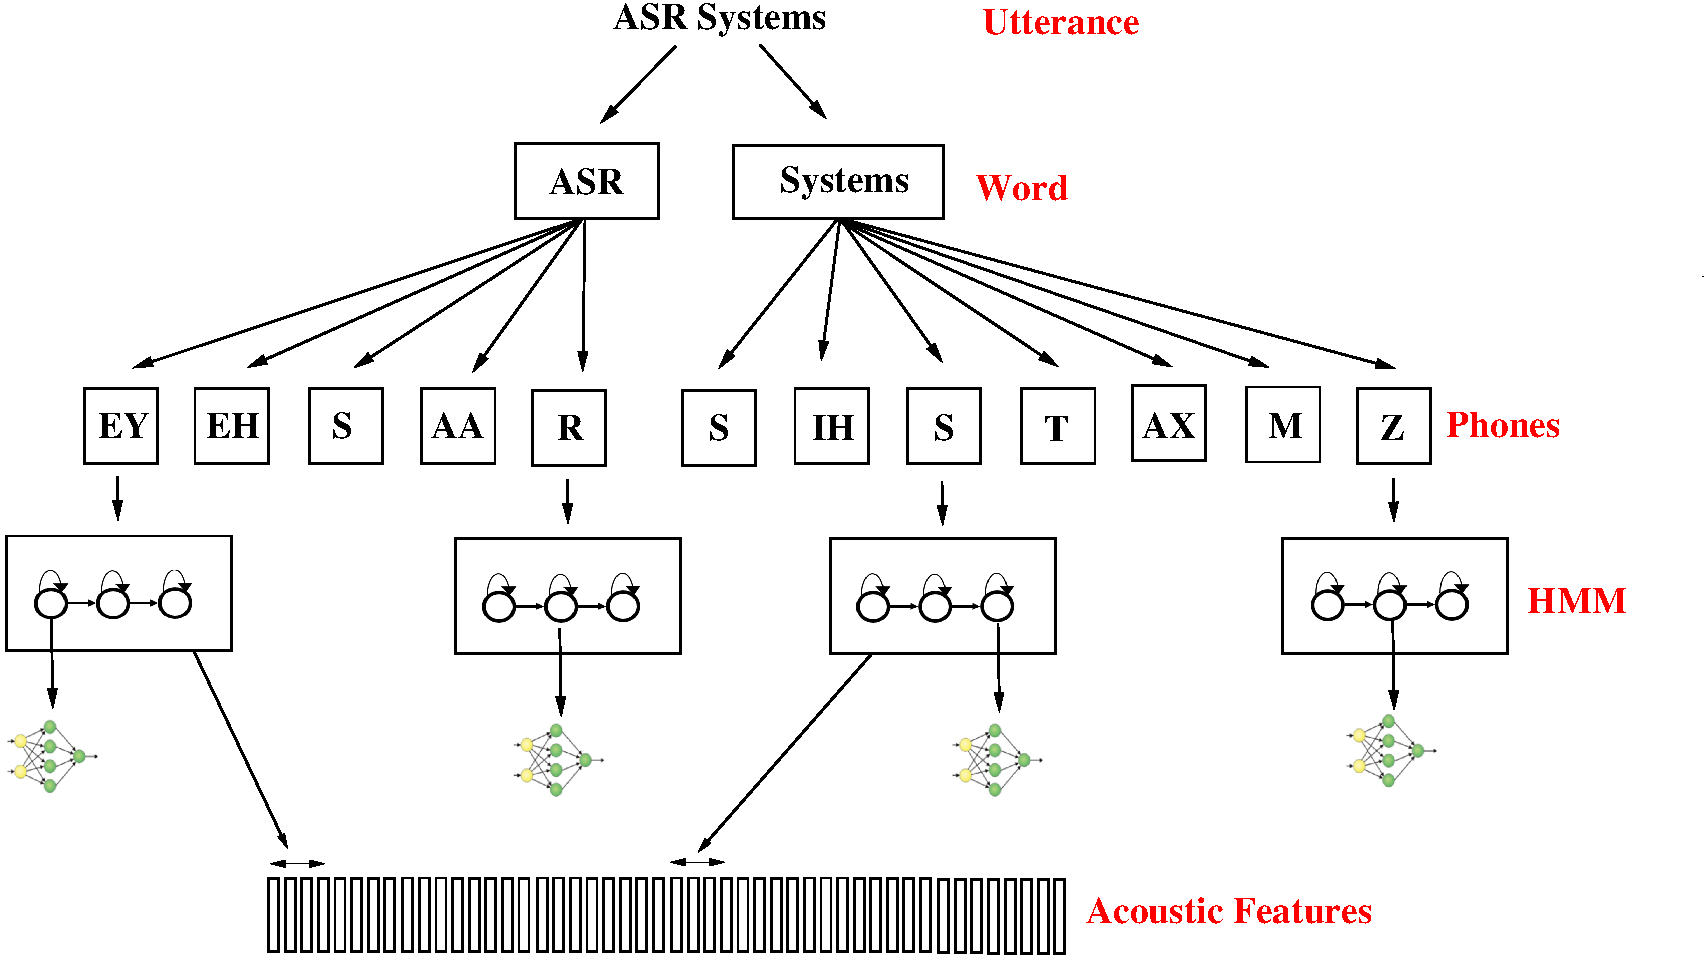
\includegraphics[height=65mm]{figures/am-mlp}
  \end{center}
\end{frame}

\begin{frame}{Challenges}
  \begin{itemize}
  \item What could be wrong?
  \item We are using a solid statistical framework
  \item We know how to extract ``features''
  \item We know how to learn models
  \item We know how to search for the best path
  \item So we must be doing the right thing!
  \end{itemize}
\end{frame}

\begin{frame}{Really? Let's think about this some more!}
  \begin{itemize}
    \item Given: an observation (ADC, FFT, ...)\\
      $\boldsymbol{X} = \boldsymbol{x}_1, \boldsymbol{x}_2, ..., \boldsymbol{x}_T$
    \item Wanted: the corresponding word sequence\\
      $W = w_1, w_2, ..., w_m$
    \item Search for the most likely word sequence $W'$
    \item Fundamental Equation of ASR: \\
      $W' = \arg \max_W P(W|\boldsymbol{X}) = \arg \max p(\boldsymbol{X}|W) P(W) $ \hspace{1cm} (Bayes)
    \item $p(\boldsymbol{X}|W)$ is the ``acoustic model''
    \item $P(W)$ is the ``language model''
    \item And how are we evaluating this?
  \end{itemize}
\end{frame}

\begin{frame}{Word Error Rate}
  \begin{itemize}
    \item \#errors / \#words (in reference)
    \item (\#insertions + \#substitutions + \#deletions) / \#words
    \item Example:\\
      \begin{tabular}{lccccc}
        Reference  &            & \texttt{SHOW} & \texttt{ME} & \texttt{THE} & \texttt{INTERFACE} \\
        Hypothesis & \texttt{I} & \texttt{SHOW} & \texttt{ME} &              & \texttt{FACE} \\
        Alignment  & \textsc{I} &               &             & \textsc{D}   & \textsc{S} \\
      \end{tabular}
    \item WER=$3/4=75\%$
    \item So? Did anyone see this in the fundamental equation? $P(W|\boldsymbol{X})$, anyone?
  \end{itemize}
\end{frame}

\begin{frame}{Fundamentals revisited}
  \begin{itemize}
  \item If we are optimizing for $P(W|\boldsymbol{X})$,
    we are optimizing for the \textit{sentence} error rate, $\langle P(W|\boldsymbol{X}) \rangle$
  \item But we want $P(\langle w_i \rangle|\boldsymbol{X})$ for $W=w_1,w_2, ..., w_m$ (for one sentence)
  \item Clearly, this is not the same thing!
  \item However, in practice, it is not complete uncorrelated either
    \begin{itemize}
    \item[$\rightarrow$] And there are ways to deal with this (confusion networks, discriminative training)
    \end{itemize}
  \item Similarly, for spoken term detection, dialog systems, etc.
  \end{itemize}
\end{frame}

\begin{frame}{The speech recogition conundrum}
  \begin{itemize}
  \item We want to optimize word error rate (or whatever)\\
    \vspace{1cm}
  \item We optimize the acoustic model for (frame-)likelihood (or cross-entropy, or MPE, sMBR, ...)
  \item We train a language model for perplexity
  \item And then we search for the most likely path (a ``sentence'')
  \item And this works?
  \end{itemize}
\end{frame}

\begin{frame}{The speech recognition conundrum - It's ugly!}
  \begin{center}
    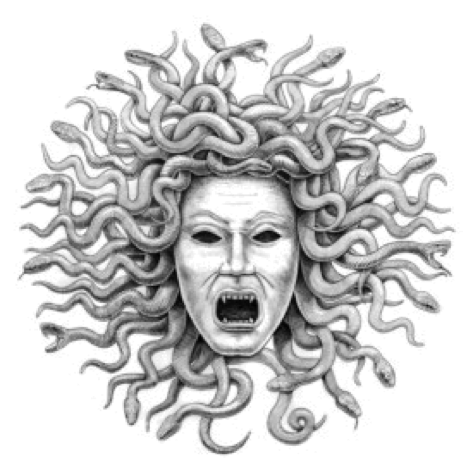
\includegraphics[height=65mm]{figures/medusa}
  \end{center}
\end{frame}

\begin{frame}{Do we really need Hidden Markov Models?}
  \begin{itemize}
  \item We know all the theory of why HMMs are good for modelling time series
  \item We have \#states, initial probability distribution, emission probabilities,
    transition probabilities, and the alphabet to define
  \item Many different ``types'' of parameters that we can play with, until we believe we have a good fit
  \item In practice, we already neglect transition probabilities
  \item The probability of staying in a state decays exponentially over time
  \end{itemize}
\end{frame}

\begin{frame}{Observed Phone Durations}
  \begin{center}
    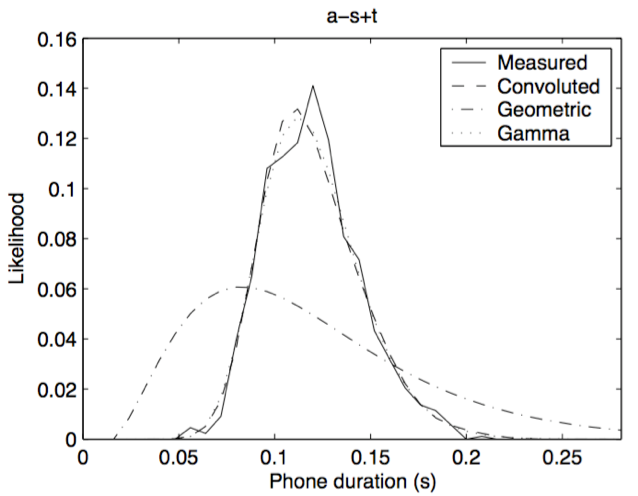
\includegraphics[height=50mm]{figures/durations}
  \end{center}
  \tiny From: \textit{Phone Duration Modeling Techniques in Continuous Speech 
    Recognition.} Janne Pylkk\"onen. Helsinki U. of Technology. 2004.
\end{frame}

\begin{frame}{Phone Durations with a single-state HMM}
  \begin{center}
    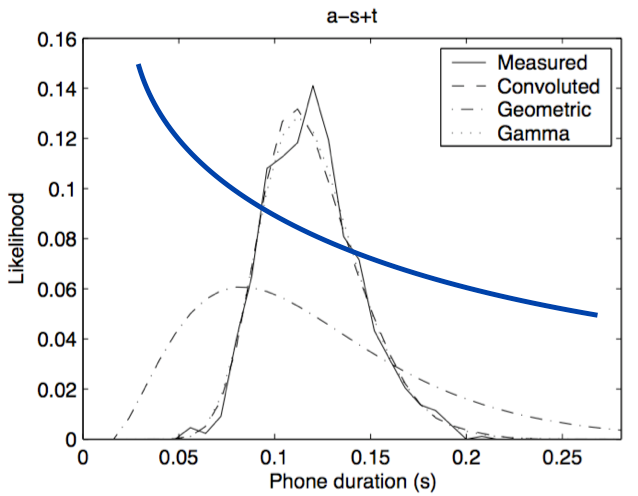
\includegraphics[height=50mm]{figures/durations3}
  \end{center}
  \begin{itemize}
  \item A single HMM state has an exponentially decreasing duration distribution.
  \item A typical tri-state topology (\textsc{-b -m -e} states) at least has a ``maximum'' peak for
    the expected duration of the whole phone
  \end{itemize}
\end{frame}

\begin{frame}{Duration Modelling with HMMs}
  \begin{itemize}
  \item A tri-state topology (-b -m -e states) at least has a ``maximum'' peak for
    the expected duration of the whole phone
  \item It is still quite arbitrary - we have plosives, short vowels, long vowels, ...\\
    \hspace{1cm}
  \item \textbf{In short}: \textit{let's not make explicit model assumptions
    that aren't really justified, and that we cannot train the parameters for}
    \begin{itemize}
    \item (I hope I am not insulting anyone, but:) duration modeling has never shown
      worthwhile, consistent gains\\
      \hspace{1cm}\\
      \hspace{1cm}
    \end{itemize}
    \item \textbf{Maybe}, \textit{we should not be using HMMs after all}
  \end{itemize}
\end{frame}

\begin{frame}{Ok, so what do we do?}
  \begin{itemize}
  \item There are a few more problems (e.g., hyper-articulation)
  \item Speech recognition ``works''
  \item Airplanes don't fly the same way birds fly
  \item We may be fine
  \item Still, what could we do?
  \end{itemize}
\end{frame}

\begin{frame}{Let's take a step back}
  \begin{itemize}
  \item What are we really trying to achieve?
  \item We want to translate a sequence of observations to a sequence of words
  \item And ideally, we want to use a single optimality criterion for that
  \item In 2016? In San Francisco?
  \end{itemize}
\end{frame}

\begin{frame}{There must be a Deep Learning solution for this!}
  \begin{center}
    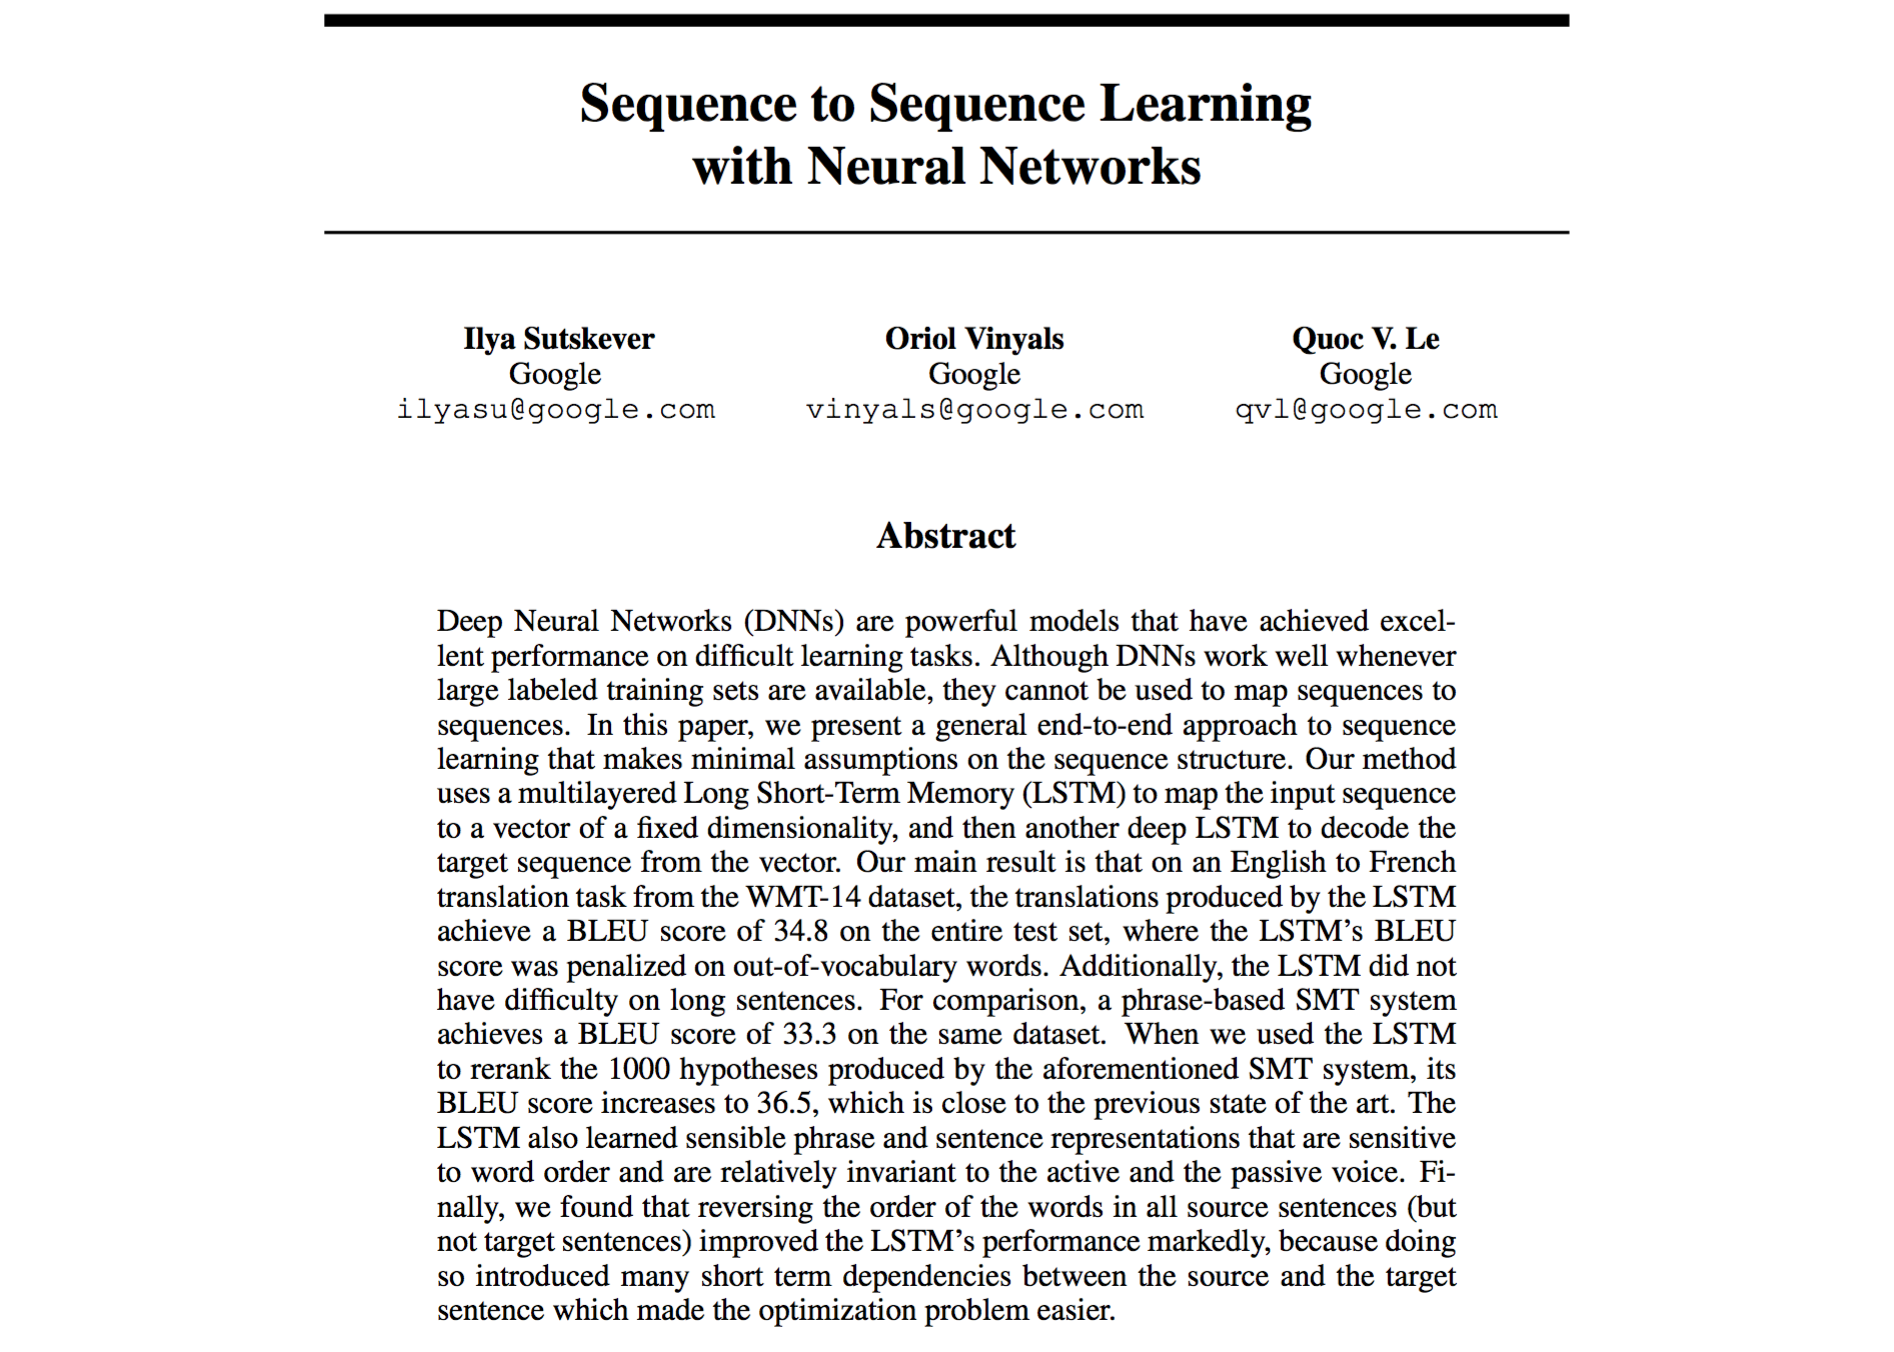
\includegraphics[height=65mm]{figures/s2s}
  \end{center}
\end{frame}

\begin{frame}
  \frametitle{Research Topics}
\end{frame}

\begin{frame}
  \frametitle{New Ideas}
\end{frame}

\begin{frame}
  \frametitle{End-to-End Systems}
\end{frame}

\section{Hands-On with Virtual Machines}

\begin{frame}
  \begin{center}
    {\color{Maroon}\Huge Hands-On Experience with Virtual Machines\par}
  \end{center}
\end{frame}

\begin{frame}
  \frametitle{Practicalities}
  \begin{itemize}
  \item We want to give you hands-on experience with building ASR systems
  \item You will be able to train a system on a Babel language (most likely 201 Haitian)
  \item You can then experiment with other Babel languages, or port the system to other domains
  \item To facilitate experimentation, we will distribute a Virtual Machine (VM)
  \item {\color{Maroon}Read on to see how you can prepare}
  \end{itemize}
\end{frame}

\begin{frame}
  \frametitle{Virtual Machines and Tools}
  \begin{itemize}
  \item Think of a VM as a ``virtual'' computer, in our case running Linux
  \item VMs allow sharing reproducible experiments easily
  \item \url{https://github.com/srvk}, \url{http://speechkitchen.org} as repositories
  \item \url{https://www.vagrantup.com/} to build VMs
  \item \url{https://www.virtualbox.org/} to run VMs (along with \url{https://aws.amazon.com/})
  \item An ``image'' is a computer when it is turned off, it becomes an ``instance'' when you turn it on
  \end{itemize}
\end{frame}

\begin{frame}
  \frametitle{Exercises}
  \begin{itemize}
  \item We will share a Vagrantfile, plus an image on AWS (most likely), and/ or a Virtualbox OVA (less likely)
  \item Your best bet is to run the exercise on AWS
  \item So, you may want to sign up for an account first (\url{https://aws.amazon.com/getting-started/})
  \item Familiarize yourself with how to start a Linux VM on ``EC2'' using a pre-configured Amazon Machine Image (AMI)
  \item Training a DNN-based recognizer on a GPU will cost some money, but the cost should not be dramatic
  \item Once you reproduced the basics, you can continue on AWS, or you can migrate to your own infrastructure
  \end{itemize}
\end{frame}

\begin{frame}
  \frametitle{Eesen}
  \begin{itemize}
  \item We will use the ``Eesen'' toolkit (\url{https://github.com/srvk/eesen}) for end-to-end speech recognition
  \item It is based on Kaldi (\url{http://kaldi-asr.org/}), but a bit smaller and easier to handle
  \item {\color{Maroon} More details to follow}
  \end{itemize}
\end{frame}

%\begin{frame}
%  \frametitle{References}    
%  \cite{quesst:icassp2015,metze:is2015,yajie-lstm:is2015,yajie-robust:is2015,yashesh:is2015,yajie:taslp2015,eesen,trecvid:2015,eesen-icassp,wang2016icassp,w4a:2016,icmr2016,miao:is2016,vms:is2016,shared:is2016,yash:is2016,e2echapter,dnnbook}
%\cite{dnnbook}
%\end{frame}
